
\documentclass{article}
%\usepackage[draft]{SRM2}
\usepackage{graphicx}
\usepackage{url}

\title{The AviaNZ Birdsong Analysis Software (v 1.0)}
\author{Stephen Marsland (\url{s.r.marsland@massey.ac.nz})}
\date{July 2017}

\usepackage[usenames, dvipsnames]{color}

\begin{document}
\maketitle

%Shift-click, ctrl-click
%scroll bar, menus not buttons

This is a brief guide to version 1.0 of the AviaNZ program. 
We really want feedback on it, particularly what works and what doesn't, how you would like to see it improved, and what other functionality it needs. We are more than happy to talk about our plans as well. 

%If you haven't done any birdsong processing before, make sure that you read Section~\ref{labelling}, which works through an example. 

When the program loads, you are presented with two options \textcolor{blue}{as shown} in the following screen:

\begin{figure}[h!]
\centering
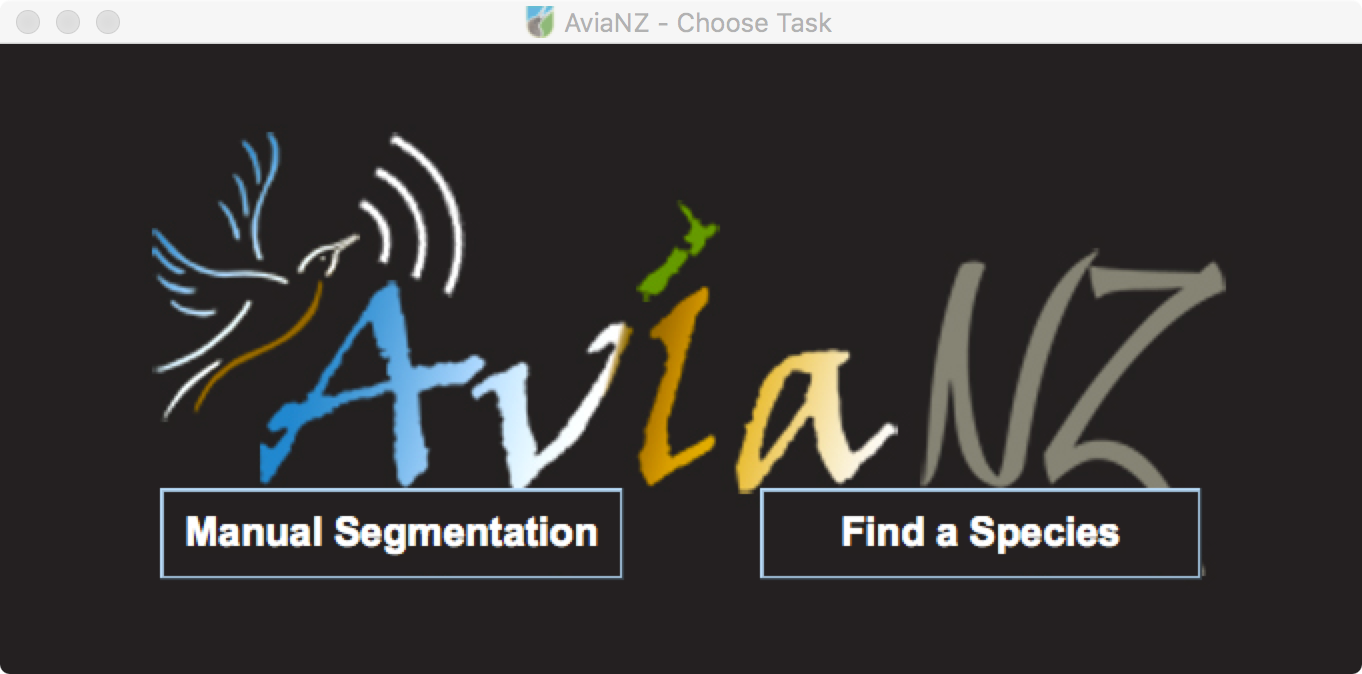
\includegraphics[width=.3\textwidth]{Figs/splashscreen}
\end{figure}

The first option (described more in Section~\ref{sec:manual}) enables you to see and manually process audio files, while the second option (see Section~\ref{sec:auto}) takes whole directories (and subdirectories) of audio files and automatically segments the bird calls of a particular species. You can then view the output of this using the first option; the software also produces an excel file showing the results (see Section~\ref{sec:outputs}).  

\section{Manual Segmentation}
\label{sec:manual}

When you select manual segmentation, you should see a dialog box asking you to select a file to view. Use this in the normal way to select a sound file from a directory. Once you have selected one, you should see a screen like the one below. This is the main program for manually labelling birdcalls, or reviewing the processing of automatic processes.
The program automatically loads the first 5 minutes of a file. 

\begin{figure}[h!]
\centering
\includegraphics[width=.8\textwidth]{Figs/avianzinterface.pdf}
\end{figure}

\begin{itemize}
\item There are five separate areas of the screen (each has its name in a blue bar). They are:
	\begin{description}
	\item[Overview] This shows you a picture of the 5 minutes of the file (labelled 2 in the figure). The part you are looking at in the main plots is shown in blue (it's actually the whole file in the example figure). Below it there is a coloured bar (labelled 3 in the figure, and in yellow). There are left and right arrow buttons (labelled 4) and double arrow buttons (labelled 5) on the left of this area. The single arrow buttons move the view in the main area along, while the double arrow buttons move to \textcolor{blue}{the previous 5 minutes or to} the next 5 minutes of the file (if it exists). 
	\item [Files (12)] This is a list of files in your current directory. You can double-click on one to select it and open it. Files in red have been annotated, files in black have not. The double arrow button on the top right of this area (labelled 11) moves on to the next file.
	\item[Amplitude plot (6)] This shows a picture of the sound file. It's one of the two parts of the interface that you can use to label the birdcalls. 
	\item[Spectrogram plot (7)] This is the second picture of the sound file, and the one that has more information and is most useful \textcolor{red}{for experts}. There is a display showing the value of the sounds at the location of the mouse (8 in the figure), and also a scroll bar to move through the file (9). \textcolor{cyan}{**I would move operator from here and label 18 from the next as they are not a part of docks**} The selected operator is shown at the bottom of the window (10).
	\item[Controls] These play the sound file, and modify the appearance of the plots (13--18 in the figure).
	\item[Menu] There is also a menu at the top of the screen. The name of the current file is shown in the title of the window (1).
	\end{description}

\item You can drag the four screen areas around and reorder them if you wish, by dragging the blue bar on the top or left of them. You can also make them into their own windows by double-clicking on the blue bar. If you decide that you made a mistake doing that, then there is an option in the Actions menu to `Put docks back' that returns them to the original configuration.

\item To load a new file, either choose `Open sound file' in the File menu, or just double click one in the Files screen area (double clicking on a folder will open that folder), or click on the button labelled 11 to move to the next file. 

\item If you want to move to a new directory, either use the `..' option at the top of the list of files to navigate around your computer's file system, \textcolor{red}{or use the  `Open sound file' in the File menu.} 

\item To quit, choose `Quit' from the File menu. 

\item The program will tell you if it is doing anything by putting text in the area labelled 18. \textcolor{blue}{The selected operator is shown at the bottom of the window (10).}

\subsection{Spectrogram and Amplitude}

\item The two main plots (Amplitude and Spectrogram; 6 and 7) show a section of a sound file. The part you are looking at is highlighted in blue in the top (Overview: 2) picture. Sometimes people only want to look at the spectrogram. If you are one of these people, in the Interface menu there is an option `Show amplitude plot', which is initially ticked. Click on it to remove the tick and the amplitude plot will vanish. If you change your mind, choose the option again. You can also hide the list of files (12) in the same way. 

\item Sometimes spectrograms don't look good initially, for example because of high noise. You can modify the brightness and contrast of the spectrogram using the two sliders marked 15 in the figure. You can also use a different colour scheme, and invert the colour map (swap black and white), by choosing the relevant options in the \textcolor{red}{Appearance }\textcolor{blue}{Interface} menu. 

\subsection{Zooming and Scrolling}

\item The part of the file you can see can be changed by:
	\begin{itemize}
	\item dragging the scroll bar below the spectrogram (9)
	\item clicking on the left or right arrows on the right of the Overview picture (labelled 4)
	\item dragging the blue highlight in the Overview picture itself (labelled 2). 
	\item clicking on any of the boxes in the bar below the Overview picture (labelled 3)
	\end{itemize}
	The amount of the file that you can see (the visible width) can be changed by either: 
	\begin{itemize}
	\item dragging the ends of that blue highlight in (2)
	\item changing the `Visible \textcolor{blue}{window width (seconds)}' in the Controls dock (labelled 17) by clicking on the up and down arrows, or typing in a new number.
	\end{itemize}

\subsection{Moving Through Long Files}

\item If files are longer than 5 minutes, use the double arrows labelled (5) to move to the next or previous sections. Note that there is a 10 second overlap between the files. \textcolor{blue}{You can also change the page size and the amount of page overlap by choosing the relevant options in the `Interface Settings' in the Interface menu.} The times on the axis below the spectrogram show locations in the full file.

\subsection{Playing the Sounds}

\item You can play the sounds visible on the screen using the `Play' button at the top-left of the Controls section (labelled 13). The button turns into a `Pause' button while playing (or you can press the `Escape' key). The light blue bar in the spectrogram plot (7)  shows where the playback is up to. You can drag this bar if you want to hear a particular part of the file. Move the mouse over it, and the bar will go red. Then click and drag to move it. The time below the play button shows the length of the file and the current position of the blue bar in minutes and seconds. You can change the volume of playback using the slider in (14). 
You can also play a segment of sound, assuming that a segment is selected. We will cover this below.

\subsection{Performing Segmentation}

\item To segment a birdcall, click the left mouse button once on either the Amplitude or Spectrogram plot. Then, as you move the mouse (within the same plot) a blue box will follow the mouse. Click again to \textcolor{red}{stop the segmentation} \textcolor{blue}{finish the segment}. The box will turn green, and a drop-down menu will then appear asking you to label the segment. 

\item Sometimes people prefer to drag boxes instead of clicking to start and stop. There is a tick box in the \textcolor{red}{Appearance} menu labelled `Drag boxes in spectrogram'. If selected, this enables you to drag a box over a frequency range {\em in the spectrogram only}. The boxes it draws are just the same as the ones by clicking, except that they highlight a particular frequency range. 

If you do this, you can use the `Make dragged boxes transparent' option to do what it says if you find the colour makes it hard to see the data.

\item If you need to add a segment on top of another one then right-click rather than left-click. This will start another segment. If dragging segments this is not a problem. 

\item To choose the type of bird, click on the name. If the type isn't in the list, move to `Other'. If it isn't in the second list, choose `Other' in this second list. It will ask you to enter a name. From then on this name will appear in the list. If you click anywhere on the screen except on a bird name in the menu then the menu will disappear and the bird type will be labelled as `Don't Know'.

\item If you click on a segment that already exists then it will turn green and the menu will reappear so that you can correct mistakes.

\item You can avoid seeing the menu by pressing the shift key on the keyboard when you click to finish the segment. The program will then give the segment the same label as the previous box that you labelled. This is very useful when there is one bird calling repeatedly.

\item You can also show that you are uncertain by pressing the control button when you click to segment (command button on a Mac computer). The names of the birds will then have a question mark after them. 

\item The segments that are drawn on the screen have different colours. They are:
	\begin{description} 
	\item[Green] This segment is currently selected. You can play it by pressing the buttons in 14, or give it a new label. 
	\item[Red] This segment has been labelled with a bird name.
	\item[Yellow] This segment has been labelled with a bird name with a question mark.
	\item[Blue] This segment has been labelled as `Don't Know'.
	\end{description}

\item These colours match the rectangles underneath the overview (labelled 3). \textcolor{blue}{By default, f}or each 10 second segment of the file, these boxes are white if there are no segments, blue if there are don't know segments, yellow if there are question marked segments, or red if all the segments in that section are labelled with definite species. \textcolor{red}{To move to a particular box,} click on it and the amplitude and spectrogram plots will show that section. 

\item Segments can be moved by dragging them, or opened out by dragging the left and right ends, just like the Overview highlight. \textcolor{blue}{For the boxes, click on the top right corner of the box and then drag to resize.}

\item Segments can be deleted by selecting them (so that they turn green) and then clicking on the `Delete Current Segment' in the Controls (16). You can also just press the \textcolor{red}{delete} key on the keyboard. 

\item To delete all of the segments, use the `Delete all segments' option in the Actions menu. 

\item Segments are saved automatically. 

\item \textcolor{blue}{You also have the flexibility to set the colors for different types of the segments as you wish. To do so navigate to `Interface settings' in the Interface menu}
\end{itemize}

\subsection{Playing a Segment}

\begin{itemize}
\item When a segment is selected (so it is green \textcolor{blue}{by default}) you can use the play button on the left of 14 in the picture to play just that small segment. You can also use the play button on the right. The difference is that the one on the right will play only the frequencies highlighted if you have dragged a limited box on the spectrogram, so that you can isolate particular frequencies of a call. \textcolor{blue}{This is particularly helpful when there is high level of background noise overlapped temporally with the sound of interest but not overlapped in the frequency domain.} 
\end{itemize}

\subsection{Menu Options}	

\subsubsection{{\em Appearance Menu}}

\begin{description}
\item [Changing appearance] The first three options in the menu hide or reveal the amplitude plot (6), list of files (12), or annotation overview (3). 
\item [Drag boxes] This option enables the user to select if they wish to perform segmentation by clicking on the start and end of a segment, or dragging a box. The boxes can be made transparent, when only their edge shows the colour code of what kind of label they have been given.
%\item[Invert Spectrogram] This is currently a play feature that shows that it is possibly to invert a spectrogram to get a new wave file. The spectrogram picture will update to be a bit blurred. 
\item [\textcolor{blue}{Choose c}olour map] This enables the user to select a colour map they prefer to the standard grey one. There is also an option to swap black and white (inverting the colour map). 
%\item [Make frequency axis tight] After bandpass filtering, this updates the spectrogram plot to stop showing the empty bands.
\item [Change spectrogram parameters] A set of `expert' options to modify the spectrogram. Enables changes of the windowing function, width and increment of the FFT, and the option to not subtract off the mean. The `Multitapering' option can make very noisy spectrograms look better, but it takes a lot of computer time. 
\item [Show fundamental frequency] Plots an estimate of the fundamental frequency for each call as a red line on the spectrogram.
\item [Make read only] When reviewing a segmentation it is possible to click on the plots by mistake, adding further segments. This option avoids this problem. It can be turned off by selecting it again. 
\item [Interface settings] \textcolor{blue}{This option enables the user to customise the annotation color scheme, cell size of the annotation overview, and auto save frequency. The user can also choose a page size. There is a tick box under `Human classify`, this option is used when reviewing the automated segmentation results  (see Section \ref{sec:action}).  There are situations that the automated detector add false positives (false alarms), then the user can delete them during the review. Here the user can save those segsments in a temporary folder for us, then we can use this information to improve the detectors. The user can add bird names to the list when annotating, but if someone wants to remove specific names from the list there is an option under Bird List. Here the user can alter the bird list by adding/deleting/changing the bird names as preferred. } 
\end{description}

\subsubsection{{\em Actions Menu}}
\label{sec:action}

These options will mostly provide dialog boxes that ask you to make choices. 

\begin{description}
\item [Delete all segments] Does what it says. 
\item [Denoise] Runs some programs that try to get rid of the noise in the sound file so that the birdcalls are easier to see. \textcolor{red}{You need to choose parameters for the algorithms.
**** We recommend using the default option, which is Bandpass plus wavelets.(?) This assumes that you know approximately the frequency range of your species of interest. ***}
\item [Segment] You can ask the computer to segment the calls automatically. 
For most users, just try the default option, and then review the output to see if you are happy with it. There are a variety of other options available, so it the default method doesn't work well, try some of those. 
 
%\item [Find Matches] If you select a segment (so that its box is green) and then press this button the program will look for others that are similar. It does not currently deal well with nosie. 
%\item [Filter Spectrogram] This tries to clean the spectrogram for easier viewing.
\item [Check Segments] These two options provide two different ways to view the segments and their labels for easier checking. The option to Show all pages decides on whether to view segments in an entire file, or just the current 5 minutes of it. 
	\begin{description}
	\item [Check segments (All segments)] This option shows the segments one-by-one in time order. 
	\begin{figure}
	\centering
	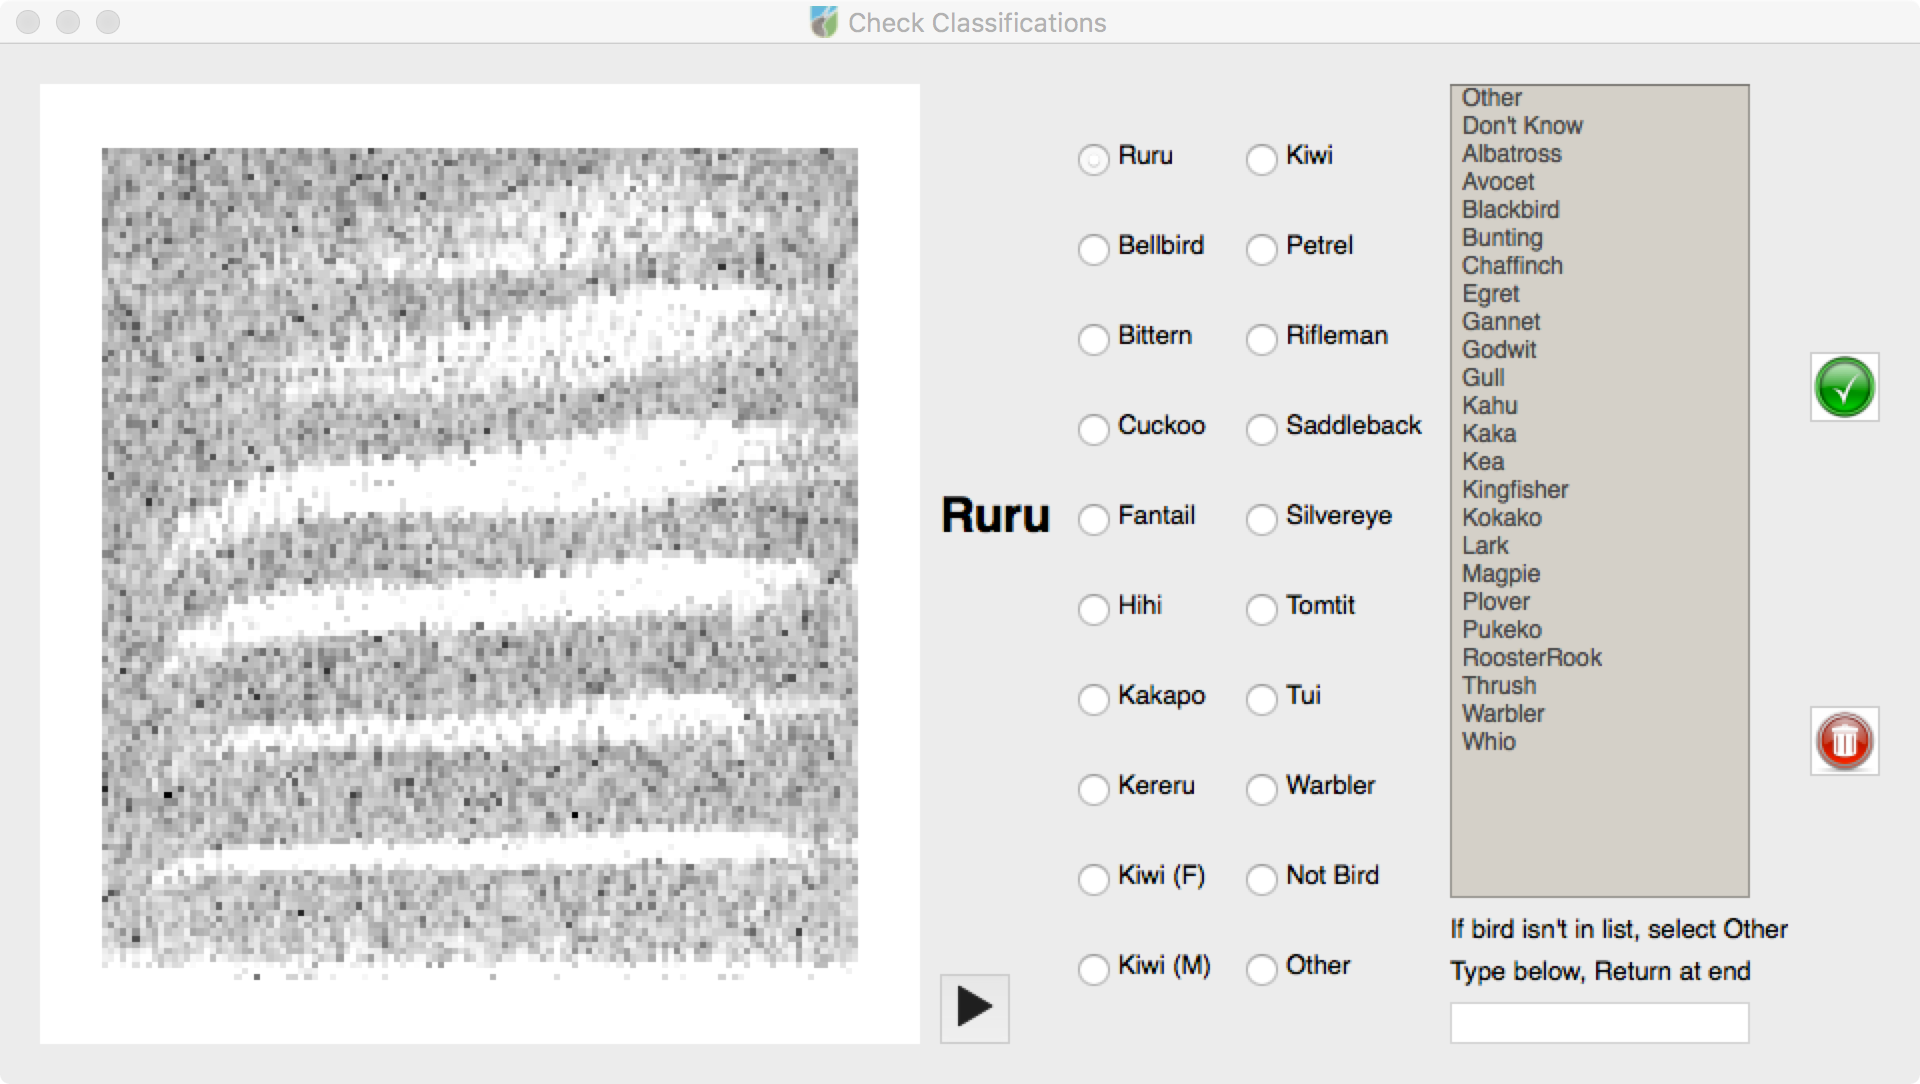
\includegraphics[width=.6\textwidth]{Figs/Check1}
	\end{figure}
	To play the segment, click on the play button. If the label is correct, click on the green tick, when the next image will load. If not, select the correct label before clicking the tick button. To delete a segment, click on the red dustbin button. 
	\item [Check segments (Choose species)] This option asks you to choose a bird from those found in the current file. For each segment that is wrongly labelled, click on its picture (the colour map will change). These segments will be deleted. 
	\begin{figure}
	\centering
	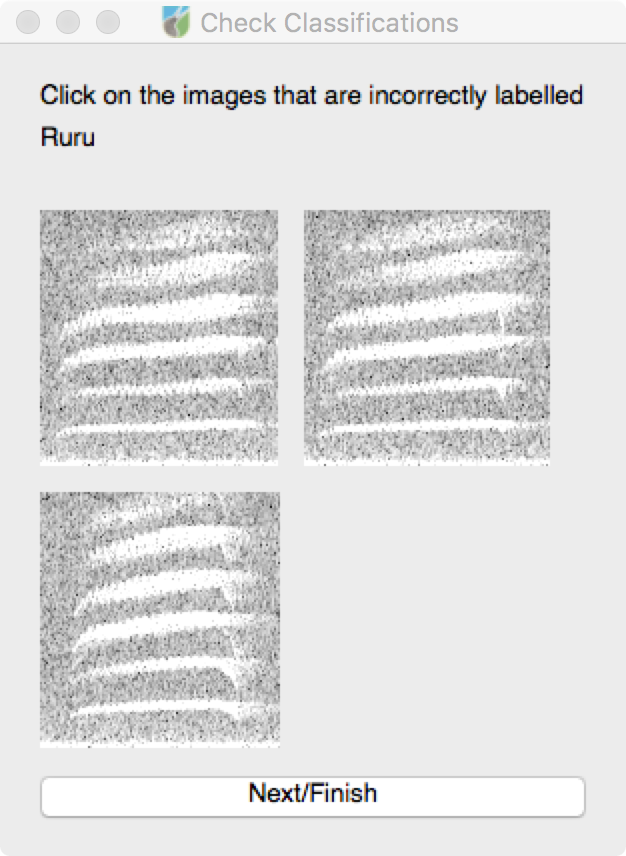
\includegraphics[width=.4\textwidth]{Figs/Check2}
	\end{figure}
	\end{description}

\item [Save as image] Saves the spectrogram currently visible on the screen as an image.
\end{description}

\subsubsection{{\em Help Menu}}

\begin{description}
\item [Help] Gives access to this file.
\item [Cheat sheet] Provides a set of examples of common bird calls. 
\end{description}


\section{Automatic Segmentation of a Folder}
\label{sec:auto}

\begin{figure}[h!]
\centering
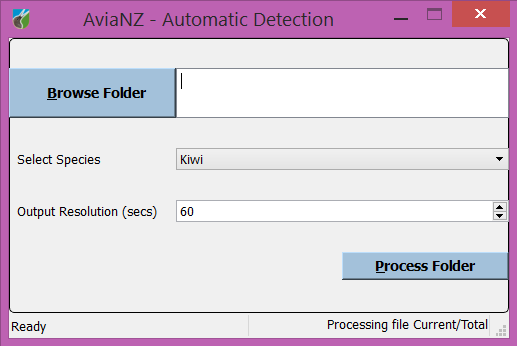
\includegraphics[width=.5\textwidth]{Figs/proc_folder}
\end{figure}

\section{Outputs}
\label{sec:outputs}

%\section{A Walkthrough}\label{labelling}
%
%This section shows you how I use the software to perform labelling. 
%
%\begin{itemize}
%\item When the program starts, choose `ruru.wav' from the list of files. This is a five minute file, and quite noisy, and it has lots of calls in it. 
%\item The two main plots show you the first 10 seconds of the recording. In the spectrogram plot, the grey speckle is noise, and the white marks inside it are the calls. Mostly people recognise the type of bird by identifying the patterns in these pictures. You should be able to see five calls, and then some noisy silence. I've highlighted the calls in this picture:
%
%\begin{figure}[h!]
%\centering
%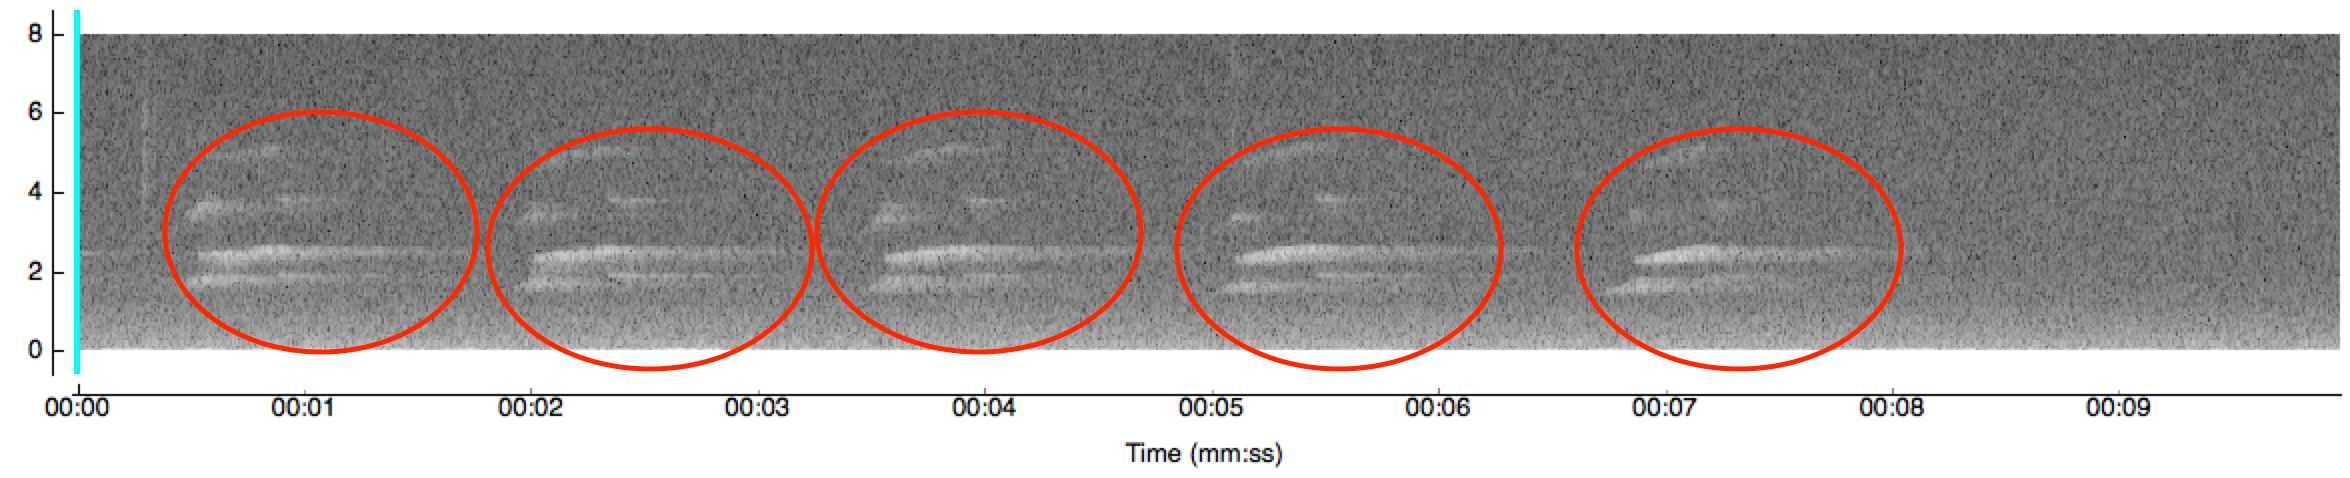
\includegraphics[width=.8\textwidth]{ruru}
%\end{figure}
%
%\item If you want to hear the calls, click on the play button (and make sure that the volume is turned up on your computer). 
%\item Play with the `Brightness' and `Contrast' sliders (12) in Figure 1 until you find it easy to see the birdcalls. If you want to make the calls be in black instead of white, click on the  `Invert colour map' option in the Appearance menu. You can also change to a different colour scheme there. I chose the options to make it look like this:
%
%\begin{figure}[h!]
%\centering
%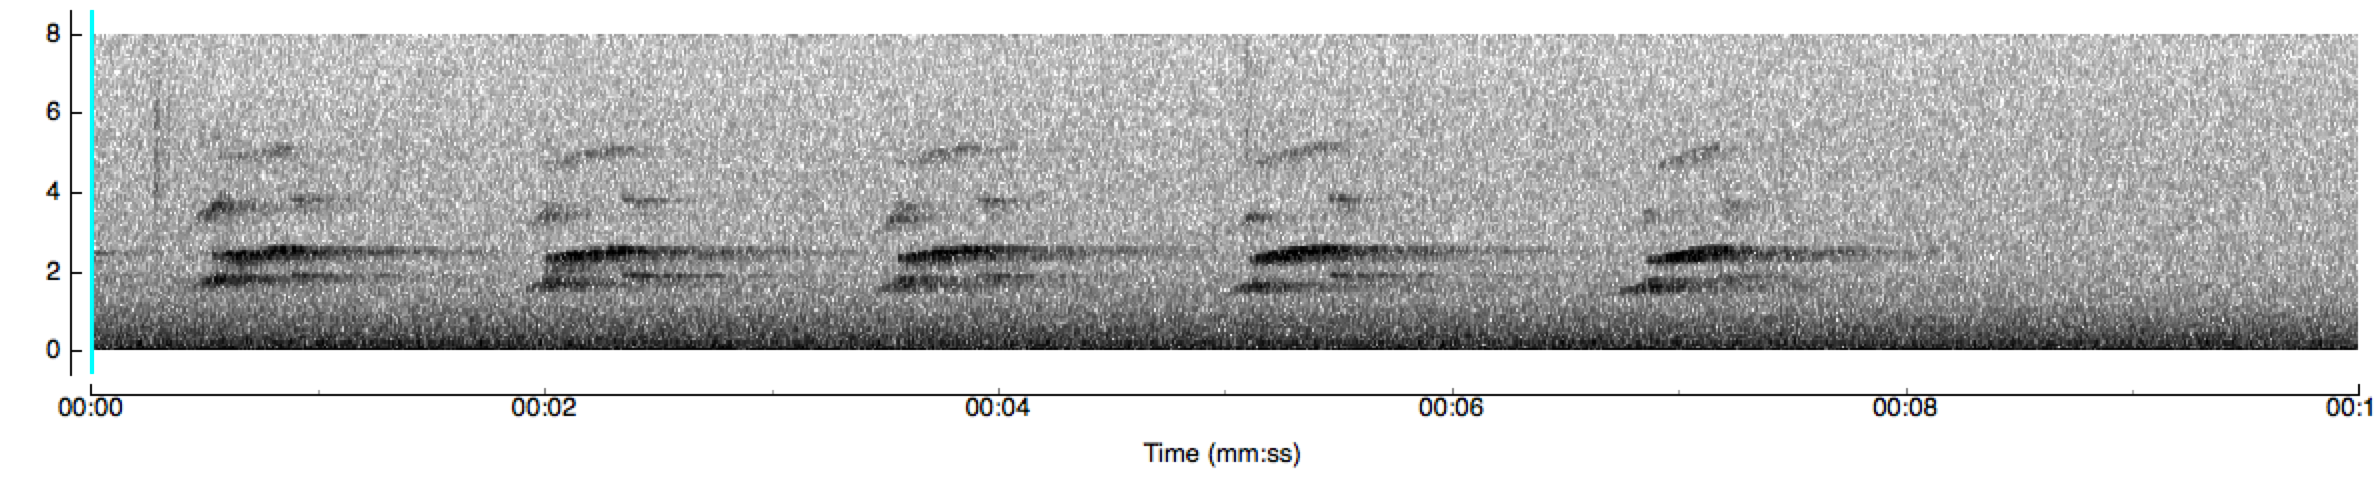
\includegraphics[width=.8\textwidth]{ruru2}
%\end{figure}
%
%\item Decide if you like seeing 10 seconds. If you prefer a different length, either: (1) drag the end of the box in the overview picture (at the top of the screen) in or out, or (2) make the length of time in `Visible window length' longer or shorter. The plots will update automatically. 
%\item Now we are ready to start to segment and label the calls. Click once with the mouse near the start of the call. Then move the mouse so that the blue box appears, and click again near the end of the call. In the drop-down box of bird names, click on `Ruru'. 
%\item If you decide you missed the start or the end, you can drag the ends of the box by putting the mouse over them, then clicking and dragging them. You can also move the whole box. 
%\item Move on to the next call and repeat.
%\item If you think that this second call is also a ruru, press shift when you click the second time, and the menu won't drop down, and the box will also be labelled as 'Ruru'
%\item If you aren't sure about a call, but think it is probably a ruru (or whatever bird) press control when you click and the menu options will have question marks on them. 
%\item When you have labelled all of the calls, press the arrow button at the top-right of the screen to move on to the next part of the recording, or drag the slider at the bottom of the screen, and carry on. 
%\item When you have finished a file, click on `Load File' to load another file, or click on `Quit' to close the program. 
%\end{itemize}
%
%When doing this you will realise what a slow and laborious procedure it is. That's why we want to automate most of it. Unfortunately, the amount of noise in the files makes it hard. You can try the different algorithms under `Segment' and see if any of them work well for your files, but for this example, which is quite noisy, they make a lot of mistakes. You can use these options and then correct the mistakes instead. Here is how:
%
%\begin{itemize}
%\item Click on `Segment' in the Actions menu. 
%\item From the list of types, choose `Median Clipping' or `Fundamental Frequency'. Ignore the parameters for now, and click on the `Segment' button below them. You might have to wait for a while. 
%\item Eventually the screen will show you lots of segment boxes. 
%\item You can delete these and move them, and label them, by clicking on them and dragging appropriately. 
%\end{itemize}

%\section{Future Plans}\label{sec:future}
%
%\begin{itemize}
%\item Quite a few things will not actually work through this interface, but through a screen before this one that asks for a directory to rip through and a species to look for in it. It will then show some outputs like the `Check Segments' outputs, except working. 
%\item Add the denoising in, ditto the wavelet segmentation, including a training phase. These are pretty much done, just need a couple of weeks.
%\item There is a whole load of feature extraction and learning algorithm work that is largely done, but isn't in this version. It's at least partly for development work at the moment, so I've kept it out of this version.
%\item <Your ideas here, please>
%\end{itemize}

\end{document}